% problemas: fundamentos de probabilidad

\section*{Problemas}

La baraja está dividida en cuatro palos (en inglés: suit), dos de color rojo y dos de color negro:
\begin{itemize}
	\item Espadas (conocidas como picas) $\spadesuit$,
	\item Corazones $\heartsuit$,
	\item Rombos (conocidos como diamantes, oros o cocos) $ \diamondsuit$,
	\item Tréboles (conocidos como flores) $\clubsuit$
\end{itemize}

Cada palo está formado por 13 cartas, de las cuales 9 cartas son numerales y 4 literales. Se ordenan de menor a mayor \emph{rango} de la siguiente forma: A, 2, 3, 4, 5, 6, 7, 8, 9, 10, J, Q y K.

\begin{figure}[ht]
	\centering
	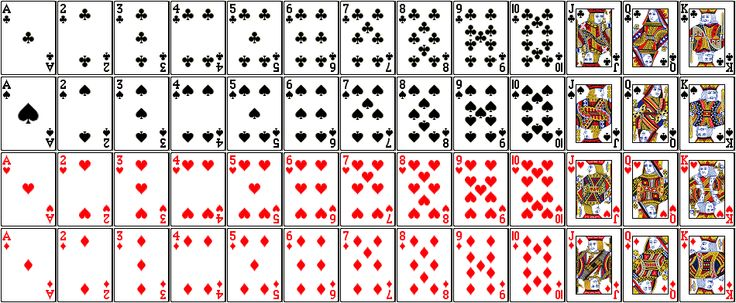
\includegraphics[width=10cm]{./pe/deck.jpg}
	\caption{Baraja inglesa}
	\label{fig:fundamentos-deck}
\end{figure}

\subsection*{Enunciados de los problemas}

% Recordar
\begin{problema}
	\label{prob:de3947a}
	Una carta se obtiene al azar de una baraja inglesa de 52 cartas. Describe formalmente el espacio muestral $S$ si se consideran los palos y los rangos.
\end{problema}

% Comprender
\begin{problema}
	\label{prob:cfa53ca}
	Supongamos que $A$ es el evento \texttt{``se obtiene un rey''} o simplemente $\set{K},$ mientras que $B$ es el evento \texttt{``se obtiene un tr\'ebol''} o simplemente $\set{\clubsuit}$. Describe con palabras el significado de los siguientes eventos combinados:
	\begin{enumerate}
		\item $A\cup B$
		\item $A\cap B$
		\item $A \cup B'$
		\item $A' \cup B'$
		\item $A - B$
		\item $A'-B'$
		\item $(A\cap B) \cup (A\cap B')$
	\end{enumerate}
\end{problema}

% Aplicar
\begin{problema}
	\label{prob:69a20ec}
	Encuéntrese la probabilidad exacta de que en dos lanzamientos de un dado balanceado de 6 caras se obtenga por lo menos un 4 en alguno de los dos lanzamientos.
\end{problema}

% Analizar
\begin{problema}
	\label{prob:1f335a1}
	A partir exclusivamente de los tres axiomas de Kolmogorov ($P(A) \ge 0$, $P(S)=1$, y aditividad para eventos mutuamente excluyentes), demuestra la regla general de adición para dos eventos arbitrarios $A, B \subset S$:
	\begin{align}
		P(A \cup B) = P(A) + P(B) - P(A \cap B).
	\end{align}
\end{problema}

% Evaluar
\begin{problema}
	\label{prob:a4ff50c}
	En una cena de gala, $n$ invitados dejan sus sombreros en el guardarropa. Al finalizar la velada, el encargado devuelve los $n$ sombreros de manera completamente aleatoria. Sea $A_{i}$ el evento de que el $i$-ésimo invitado reciba su propio sombrero ($i=1,2,\dots,n$).
	\begin{enumerate}
		\item Utilizando el principio de inclusión-exclusión para probabilidades, evalúa y demuestra la fórmula general para la probabilidad de que \emph{al menos uno} de los invitados reciba su sombrero correcto:
		\begin{align}
			P\left( \bigcup_{i=1}^{n} A_{i} \right) = \sum_{k=1}^{n} \frac{(-1)^{k-1}}{k!}.
		\end{align}
		\item Calcule el límite de esta probabilidad cuando el número de invitados crece indefinidamente ($n \to \infty$) y juzgue por qué el resultado es contraintuitivo.
	\end{enumerate}
\end{problema}

% Crear
\begin{problema}
	\label{prob:b993271}
	Diseñe un experimento aleatorio original (distinto de cartas, dados o sombreros) con un espacio muestral $S$ de al menos 8 puntos muestrales equiprobables, y defina sobre él dos eventos $A$ y $B$ no disjuntos. Calcule $P(A)$, $P(B)$, $P(A \cap B)$ directamente por conteo, y verifique numéricamente que su resultado satisface la regla general de adición $P(A \cup B) = P(A) + P(B) - P(A \cap B)$.
\end{problema}

\subsection*{Soluciones detalladas}

% Recordar
\begin{solproblema}[prob:de3947a]
	La solución está dada por el producto cartesiano del conjunto de palos:
	\begin{align}
		P = \set{\spadesuit, \heartsuit, \diamondsuit, \clubsuit},
	\end{align}
	cuya cardinalidad es 4, y el conjunto de rangos:
	\begin{align}
		R = \set{\text{A}, 2, 3, 4, 5, 6, 7, 8, 9, 10, \text{J}, \text{Q}, \text{K}},
	\end{align}
	cuya cardinalidad es 13. El espacio muestral completo es $S = P \times R$, conteniendo exactamente $4 \times 13 = 52$ puntos muestrales equiprobables.
\end{solproblema}

% Comprender
\begin{solproblema}[prob:cfa53ca]
	\begin{enumerate}
		\item $A \cup B$: Se obtiene un rey o un trébol (o ambos).
		\item $A \cap B$: Se obtiene simultáneamente un rey y un trébol (específicamente, el Rey de Tréboles).
		\item $A \cup B'$: Se obtiene un rey o no se obtiene un trébol (equivalente a: si es trébol, necesariamente es rey).
		\item $A' \cup B'$: No se obtiene un rey o no se obtiene un trébol (por Ley de De Morgan, es el complemento de obtener el Rey de Tréboles).
		\item $A - B$: Se obtiene un rey que no es de trébol ($A \cap B'$).
		\item $A' - B'$: No se obtiene rey y además sí se obtiene trébol ($A' \cap B$).
		\item $(A \cap B) \cup (A \cap B')$: Se obtiene un rey que es de trébol o un rey que no es de trébol. Por distributividad de la intersección respecto a la unión, esto equivale simplemente al evento $A$ (\texttt{``se obtiene un rey''}).
	\end{enumerate}
\end{solproblema}

% Aplicar
\begin{solproblema}[prob:69a20ec]
	El espacio muestral del lanzamiento de dos dados consta de $6 \times 6 = 36$ pares ordenados equiprobables. Calculamos por el evento complementario: el evento $E'$ de \emph{no} obtener ningún 4 en ninguno de los dos dados significa que cada dado puede caer en cualquiera de las 5 caras restantes ($\{1,2,3,5,6\}$).

	El número de casos favorables para el complemento $E'$ es $5 \times 5 = 25$. Por lo tanto, la probabilidad del evento $E$ (\texttt{``al menos un 4''}) es:
	\begin{align}
		P(E) = 1 - P(E') = 1 - \dfrac{25}{36} = \dfrac{11}{36} \approx 0.3056.
	\end{align}
\end{solproblema}

% Analizar
\begin{solproblema}[prob:1f335a1]
	A partir de la teoría de particiones, podemos expresar el conjunto unión $A \cup B$ y el conjunto $B$ como uniones de conjuntos mutuamente excluyentes (disjuntos):
	\begin{align}
		A \cup B &= A \cup (B \backslash A) \\
		B &= (A \cap B) \cup (B \backslash A)
	\end{align}
	Por el tercer axioma de Kolmogorov (aditividad numerable para conjuntos disjuntos):
	\begin{align}
		P(A \cup B) &= P(A) + P(B \backslash A) \label{eq:fundprob_u1} \\
		P(B) &= P(A \cap B) + P(B \backslash A) \implies P(B \backslash A) = P(B) - P(A \cap B) \label{eq:fundprob_u2}
	\end{align}
	Sustituyendo la ecuación (\ref{eq:fundprob_u2}) en la ecuación (\ref{eq:fundprob_u1}):
	\begin{align}
		P(A \cup B) = P(A) + P(B) - P(A \cap B).
	\end{align}
	Esta identidad demuestra la regla general de adición en probabilidad sin depender de conteos finitos.
\end{solproblema}

% Evaluar
\begin{solproblema}[prob:a4ff50c]
	\begin{enumerate}
		\item La probabilidad de que una persona reciba su sombrero correcto es la relación entre permutaciones que fijan al menos un elemento. Para un índice individual $i$, $P(A_i) = \frac{(n-1)!}{n!} = \frac{1}{n}$. Para dos personas $i < j$, $P(A_i \cap A_j) = \frac{(n-2)!}{n!} = \frac{1}{n(n-1)}$. En general, para la intersección de $k$ personas simultáneas, la probabilidad es $\frac{(n-k)!}{n!}$.

		El principio general de inclusión-exclusión para $n$ eventos establece:
		\begin{align}
			P\left( \bigcup_{i=1}^{n} A_i \right) = \sum_{i=1}^n P(A_i) - \sum_{i<j} P(A_i \cap A_j) + \dots + (-1)^{n-1} P(A_1 \cap \dots \cap A_n).
		\end{align}
		El número de formas de elegir $k$ personas de un total de $n$ es $\binom{n}{k}$. Multiplicando la probabilidad conjunta por el número de combinaciones en el término $k$-ésimo:
		\begin{align}
			S_k = \binom{n}{k} \cdot \frac{(n-k)!}{n!} = \frac{n!}{k!(n-k)!} \cdot \frac{(n-k)!}{n!} = \frac{1}{k!}.
		\end{align}
		Sustituyendo cada suma parcial $S_k$ en la fórmula principal:
		\begin{align}
			P\left( \bigcup_{i=1}^{n} A_i \right) = \sum_{k=1}^{n} (-1)^{k-1} S_k = \sum_{k=1}^{n} \frac{(-1)^{k-1}}{k!}.
		\end{align}

		\item Recordemos la serie de Taylor para la función exponencial evaluada en $x = -1$:
		\begin{align}
			e^{-1} = \sum_{k=0}^{\infty} \frac{(-1)^k}{k!} = 1 - \sum_{k=1}^{\infty} \frac{(-1)^{k-1}}{k!}.
		\end{align}
		Por lo tanto, cuando el número de invitados crece ($n \to \infty$):
		\begin{align}
			\lim_{n \to \infty} P\left( \bigcup_{i=1}^{n} A_i \right) = 1 - e^{-1} \approx 0.63212.
		\end{align}
		El resultado es contraintuitivo porque es \emph{independiente del tamaño de la cena}: ya sea con $n=10$ o $n=10{,}000$ invitados, la probabilidad de que al menos uno reciba su propio sombrero se estabiliza de manera prácticamente idéntica en $63.21\%$ a partir de $n \ge 6$, en contra de la intuición de que agregar más invitados debería diluir la probabilidad de una coincidencia.
	\end{enumerate}
\end{solproblema}

% Crear
\begin{solproblema}[prob:b993271]
	\textbf{Ejemplo:} un dado balanceado de 8 caras (numeradas 1 a 8) se lanza una vez, de modo que $S=\{1,2,\dots,8\}$ con $8$ puntos equiprobables. Sea $A=\{2,3,4,5\}$ (\texttt{``el resultado es par o impar entre 2 y 5''}) y $B=\{4,5,6,7\}$ (\texttt{``el resultado está entre 4 y 7''}), que no son disjuntos porque $A\cap B=\{4,5\}$.

	Por conteo directo:
	\begin{align}
		P(A) = \frac{4}{8}=0.5, \qquad P(B) = \frac{4}{8}=0.5, \qquad P(A\cap B) = \frac{2}{8}=0.25.
	\end{align}
	La unión es $A\cup B=\{2,3,4,5,6,7\}$, con $P(A\cup B)=6/8=0.75$ por conteo directo. Verificando con la regla general de adición:
	\begin{align}
		P(A) + P(B) - P(A\cap B) = 0.5+0.5-0.25 = 0.75 = P(A\cup B),
	\end{align}
	confirmando que el conteo directo y la fórmula coinciden exactamente.
\end{solproblema}
